\section{项目的主要内容和技术路线}

\subsection{主要研究内容}

本研究主要围绕对抗性偏好优化算法的设计与实现展开,通过引入对抗性训练机制,结合数据扩展和自我优化策略,构建一个高效的偏好优化框架。核心思想是通过偏好反馈生成数据集,
并在此基础上进行自标注和多轮迭代优化,从而提升模型的对齐效果。特别地,
采用对抗性训练帮助模型在面对噪声数据时进行自我纠正,确保其在数据稀缺的情况下仍能保持高效的对齐。
此外,希望形成一种结合数据扩展和自我优化策略的方法,通过现有的初始模型或参考模型生成更多的偏好反馈数据,
并利用自我优化策略对这些数据进行多轮优化,以进一步提升模型的任务适应性和对齐度。

本研究的实验部分将通过一系列验证,展示该算法在数据稀缺和标注困难的应用场景中的有效性,
尤其是在减少人工标注数据需求的同时,如何显著提升模型的对齐度和鲁棒性。

\subsection{技术路线}

\subsubsection{对抗性偏好学习框架}

本项目的大致算法框架如下:
\begin{enumerate}
    \item 模型策略:大语言模型在训练时试图选择一条策略$\pi$,以最大化在各种反馈分布下的期望奖励。
    \item 偏好分布:假设存在一个最坏情况或对抗性的偏好分布,会根据模型策略来挑选最具挑战性的输入或偏好标注。
    \item 对抗过程:在给定策略下做对抗性反馈响应,模型通过在最不利的偏好条件下依然优化奖励,从而获得鲁棒性与普适性。
\end{enumerate}
对于最坏分布,考虑构造关于偏好数据对奖励的经验分布,在其 Wasserstein 距离不超过 $\epsilon$(给定超参数)下寻找
最可能降低模型奖励期望的偏好分布。这里我们认为“最具有挑战性”的数据指的是目前模型最易混淆的偏好数据对。

\begin{figure}[h]
    \centering
    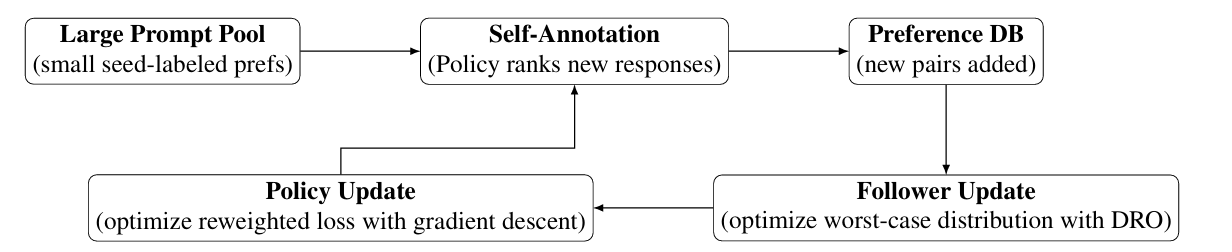
\includegraphics[width=0.95\textwidth]{figure/SSAPO.png}
    \caption{算法流程图}
\end{figure}

\subsubsection{最坏分布求解方法} \label{sec:bad-dis}

原始的 DPO 训练过程只考虑优化现有样本的经验分布,在样本数量较少的情况下容易出现过拟合的现象。
在对抗性训练中,需要基于当前的数据经验分布构造一个使得模型期望奖励最低的“最坏分布”,
对于这个任务,我考虑采用论文 DRO\citep{Esfahani2018Data} 的技术路线,
将求解过程看作一个高维随机规划问题。在温和假设下,Wasserstein球上的分布随机优化问题实际上可以被重新表述为有限凸规划——在许多有趣的情况下,甚至可以作为可处理的线性规划。

设偏好数据分布为 $(x, y_w) \sim \mathcal{D}_w$,非偏好数据分布为 $(x, y_l) \sim \mathcal{D}_l$,其联合分布为 $\mathcal{D}$,样本集为 $D_n = \{(x, y_w, y_l)\}_1^N$。
训练的优化的目标为:(其中 $\theta$ 是模型的参数)
\begin{equation}
    J^* := \inf_{\theta \in \Theta} \left\{ \mathbb{E}^{\mathcal{D}} [h(\theta, x,y_w,y_l)]\right\}
\end{equation}
其中 $h(\theta, x, y_w, y_l) = - \left[ \log \sigma \left( \beta \log \dfrac{\pi_{\theta}(y_w | x)}{\pi_{\text{ref}} (y_w |x)} -  \beta \log \dfrac{\pi_{\theta}(y_l | x)}{\pi_{\text{ref}} (y_l |x)} \right)\right]$  

我们考虑对问题进行适当的简化,在固定模型参数 $\theta$ 的情况下,定义
\begin{equation}
    \xi = \sigma \left( \beta \log \dfrac{\pi_{\theta}(y_w | x)}{\pi_{\text{ref}} (y_w |x)} -  \beta \log \dfrac{\pi_{\theta}(y_l | x)}{\pi_{\text{ref}} (y_l |x)} \right)
\end{equation}
$\xi \in \Xi$ 的边际分布可以由数据的经验分布 $\hat{\mathcal{D}}_N$ 导出,设为 $\hat{P}_N$,
我们的目标是求解其 Wasserstein $\epsilon$-临域 $\tilde{\mathcal{P}}_N := \mathbb{B}_{\epsilon}(\hat{P}_N)$ 内最坏分布的目标期望:
\begin{equation}
    \sup_{\mathbb{Q} \in \tilde{\mathcal{\mathcal{P}}}_N} \mathbb{E}^{\mathbb{Q}} [\ell (\xi)] : \ell(\xi) = - \log \xi
\end{equation}

假设不确定域 $\Xi\subseteq \mathbb{R}$ 是凸且闭的。
且假设 $\ell(\xi) = \max_{k=1}^K \ell_k(\xi)$,其中 $\ell_k(\xi), k = 1, \cdots, K$ 是一系列凹函数,换言之,
$\ell(\xi)$ 可以用一些列凹函数的 pointwise-maximun 表示(这样的假设并不会引入过多的限制)。
最简单的,我们可以使用线性函数来构造 $\ell(\xi) =  - \log \xi$ 的下凹包,可以证明该方法是对损失函数的一个良好近似。
参考\citep{Esfahani2018Data}的证明过程,我们可以证明构造最坏分布等价于求解如下有限凸优化问题:
\begin{equation}
    \begin{aligned}\sup_{\alpha_{i,k}, q_{i,k}} &  \frac1N \sum_{i=1}^N \sum_{k=1}^K \alpha_{i,k} \ell_{k} (\xi_i - \frac{q_{i,k}}{\alpha_{i,k}}) \\ \text{s.t.} & \frac1N \sum_{i=1}^N\sum_{k=1}^K \| q_{i,k} \| \leq \varepsilon \\ & \sum_{k=1}^K \alpha_{i,k} = 1 & \forall i \leq N \\ & \alpha_{i,k} \geq 0 & \forall i\leq N, \forall k \leq K \\  & \xi_i - \frac{q_{i,k}}{\alpha_{i,k}} \in \Xi & \forall i \leq N, \forall k \leq K \end{aligned}
\end{equation}

% 定义经验分布为: $\hat{\mathcal{D}}_N := \frac1N \sum_{i=1}^N \delta_{(x, y_l, y_w)}$,
% 其 Wasserstein 度量下的 $\epsilon$-邻域为 $\tilde{\mathcal{D}}_N$,目标是最优化邻域内最坏分布的目标期望:
% \begin{equation}
%     \hat{J}_N := \inf_{\theta \in \Theta} \sup_{\mathbb{Q} \in \tilde{\mathcal{D}}_N} \mathbb{E}^{\mathbb{Q}} [h(\theta, x, y_w ,y_l)]
% \end{equation}

% 在固定 $\theta$ 的情况下,定义 $\xi = \sigma \left( \beta \log \dfrac{\pi_{\theta}(y_w | x)}{\pi_{\text{ref}} (y_w |x)} -  \beta \log \dfrac{\pi_{\theta}(y_l | x)}{\pi_{\text{ref}} (y_l |x)} \right)$,其边际分布可以由 $\hat{\mathcal{D}}_N$ 导出,设为 $\hat{P}_N$,求解邻域 $\tilde{\mathcal{P}}_N := \mathbb{B}_{\epsilon}(\hat{P}_N)$  内最坏分布的目标期望:
% \begin{equation}
%     \sup_{\mathbb{Q} \in \tilde{\mathcal{\Xi}}_N} \mathbb{E}^{\mathbb{Q}} [\ell (\xi)]
% \end{equation}

% 现假设不确定域( $\mathcal{D}$ 的支持集) $\Xi \in \mathbb{R}^m$ 是凸且闭的,

对应最坏分布为:
\begin{equation}
    \mathbb{Q}_r := \frac1N \sum_{i=1}^N \sum_{k=1}^K \alpha_{i,k} \delta_{\xi_i - \frac{q_{i,k}}{\alpha_{i,k}}}
\end{equation}
其中 $r$ 为迭代步数,在分布的轻尾假设条件下,可以证明 $r\to \infty, \mathbb{E}^{\mathbb{Q}_r} [\ell] \to\sup_{\mathbb{Q} \in \tilde{\mathcal{D}}_N} \mathbb{E}^{\mathbb{Q}} [\ell]$。
这样我们就把最坏分布的构造这样一个高维随机规划转化为一个简单的凸优化问题。

\subsubsection{在重加权数据上的训练}

多轮训练过程可以参考 SPA\citep{kim2025spread} 论文中的算法框架,利用模型自生成自标注数据,经过 \ref{sec:bad-dis} 构造最坏分布,
采用 DPO\citep{rafailov2023direct}的训练范式对重加权数据进行训练。

根据\ref{sec:bad-dis},我们修改DPO的训练目标为如下形式:
\begin{equation}
    \mathcal{L}_{\text{DPO}} = \sum_{i=1}^N \sum_{k=1}^K -\log  \left[\alpha_{i,k}\left( \sigma \left( \beta \log \dfrac{\pi_{\theta}(y_w | x)}{\pi_{\text{ref}} (y_w |x)} -  \beta \log \dfrac{\pi_{\theta}(y_l | x)}{\pi_{\text{ref}} (y_l |x)} \right)- \frac{q_{i,k}}{\alpha_{i,k}}\right)\right] 
\end{equation}

\subsection{可行性分析}

首先,从理论可行性来看,迭代自增强模型已经在多个研究中证明了其有效性\citep{Kim2025Spread},表明通过不断更新模型并利用其自身生成的偏好数据进行优化,能够显著提升模型的对齐性能。此外,分布鲁棒优化(DRO)\citep{Esfahani2018Data} 提供了一种有效的框架来求解最坏情况下的偏好分布问题,其中高维随机规划问题可以等价转化为线性规划问题,降低了计算复杂度。针对凹凸性假设,可以使用线性函数拟合损失函数,从而保证最坏分布的可计算性。由于 DRO 已经在多个优化问题中得到成功应用,其方法在本研究中的适用性具有较强的理论支撑。

其次,从计算可行性来看,求解最坏分布通常是 DRO 方法的核心挑战,但已有研究表明,在适当的假设下,这一问题可以通过高效的线性规划求解\citep{Esfahani2018Data}。特别是当数据量较大时,可以采用分组策略,以保证计算的可扩展性。结合高性能并行计算技术,优化过程可以在可接受的时间范围内完成,从而确保在大规模数据集上的训练效率。此外,现有的分布式计算框架(如 GPU 并行优化和参数服务器架构)可以进一步加速 DRO 求解,使得模型能够在实际应用场景中具备高效训练的能力。

最后,从实际应用可行性来看,当前基于 DPO 的方法已经展示了较好的偏好对齐能力,而本研究进一步结合自增强学习与对抗性优化,使得模型在减少人工标注需求的同时,也能提升对抗噪声数据的鲁棒性。这种方法适用于大规模真实世界场景,特别是人工标注数据昂贵且存在一定噪声的任务。在实际应用中,可以通过迭代自增强机制逐步优化偏好数据的质量,使得模型在较少的人类监督下依然能够达到高水平的对齐效果。
